%\pagenumbering{arabic}
%\setcounter{page}{1}
\setcounter{chapter}{11}
\chapter{One Sample Hypothesis Test on a Proportion and Variance}
%\index{Introduction}
%\label{sec.matrix}
%start relabeling as 2.1 etc
%\pagestyle{myheadings}  \markboth{\ref{sec.matrix}.
%\titleref{sec.matrix}}{}
%\setcounter{equation}{0}

Inferential statistics is a powerful method for statistical analysis, because it allows people to analyze a lot parameters. Similarly to confidence interval, testing hypothesis can be applied to proportion and variance as well. Also, we use the exact same structure for one sample hypothesis test on a proportion and variance.

\section{One Sample Hypothesis Test on a Proportion}

Suppose we have assume the proportion of a criteria from a population $p$ is equal to our parameter $p_0$ (null hypothesis $H_0: p = p_0$). While, the question is: how do we know whether our assumption is correct or not? We need to use testing hypothesis on proportion to verify. \\

\textbf{Step 1: Stating the Structure of Testing Hypothesis}

First of all, let's proceed with a table to see all the cases:

\begin{center}
\begin{figure}[H]
\centering
\begin{tabular}{ c c c }
Cases & Null Hypothesis & Alternative Hypothesis \\
     1	   & $H_0: p = p_0$ & $H_a: p > p_0$ \\
     2	   & $H_0: p = p_0$ & $H_a: p < p_0$ \\
     3    & $H_0: p = p_0$ & $H_a: p \neq p_0$ \\
\end{tabular}
\caption{All possible cases of one sample hypothesis test on a proportion ($p$ represents the actual proportion of a population)}
\end{figure}
\end{center}
\vspace{-0.75cm}
We are not going to proceed with all three cases in a single question. You need to be able to identify which case of testing hypothesis are going to be applied from question.\\

\textbf{Step 2: Computing Test Statistics}

After that we need to compute our test statistics, as the following definition provides:

\begin{definition}[Test statistics of one sample hypothesis test on a proportion]
The test statistics of one sample hypothesis test on a proportion is given by: \[ Z^* = \frac{\hat{p} - p_0}{ \sqrt{ \frac{p_0(1-p_0)}{n} } } \]
In this case, $n$ means the sample size, $\hat{p}$ is the parameter of the proportion of the population, which is calculated by $\hat{p} = \frac{\text{number of successes in the sample}}{n}$. Also, the reference distribution is standard normal distribution: $N(0,1)$.
\end{definition}

Note that be careful while you are computing the test statistics, because it directly affects the final answer.\\

\textbf{Step 3: Finding the $p$ - value}

Case 1: $H_0: p = p_0$, $H_a: p > p_0$:

i. When is structure of testing hypothesis is $H_0: p = p_0$, $H_a: p > p_0$:

\begin{figure}[h]
\begin{center}
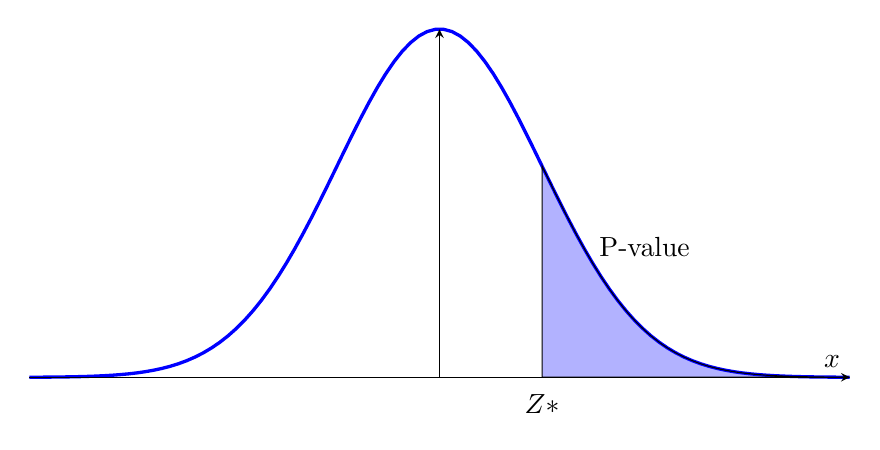
\begin{tikzpicture}
  \begin{axis}[
    no markers, domain=-4:4, samples=100,
    axis lines=middle,
    xlabel={$x$}, ylabel={},
    height=6cm, width=12cm,
    xtick=\empty,
    ytick=\empty,
    enlargelimits=false, clip=false,
    axis on top,
    grid = major,
  ]
    \addplot [very thick, blue] {1/sqrt(2*pi) * exp(-x^2/2)};
    \addplot [
      domain=1:4,
      samples=100,
      fill=blue,
      fill opacity=0.3,
    ]
    {1/sqrt(2*pi) * exp(-x^2/2)} \closedcycle;
     \node at (axis cs:2, 0.15) {P-value};
     \node at (axis cs:1, -0.03) {$Z*$};
  \end{axis}
\end{tikzpicture}
\end{center}
\caption{An illustration of hypothesis test on a proportion that $H_0: p = p_0$, $H_a: p > p_0$.}
\end{figure}

Just like one same hypothesis test on a mean from previous chapter, the p-value in the case when $H_0: p = p_0$, $H_a: p > p_0$ is the probability under the standard normal cure where the area greater than your test statistics: p-value $= P(X \ge Z^*)$.\\

Case 2: $H_0: p = p_0$, $H_a: p < p_0$:

\begin{figure}[H]
\begin{center}
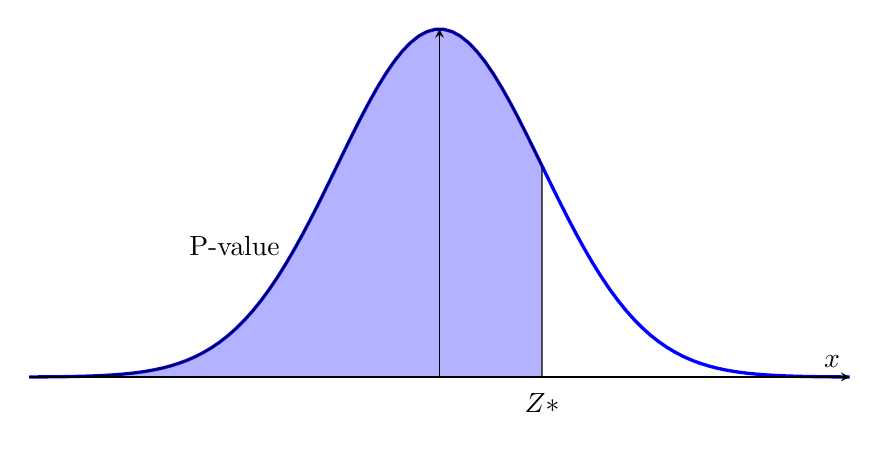
\begin{tikzpicture}
  \begin{axis}[
    no markers, domain=-4:4, samples=100,
    axis lines=middle,
    xlabel={$x$}, ylabel={},
    height=6cm, width=12cm,
    xtick=\empty,
    ytick=\empty,
    enlargelimits=false, clip=false,
    axis on top,
    grid = major,
  ]
    \addplot [very thick, blue] {1/sqrt(2*pi) * exp(-x^2/2)};
    \addplot [
      domain=-4:1,
      samples=100,
      fill=blue,
      fill opacity=0.3,
    ]
    {1/sqrt(2*pi) * exp(-x^2/2)} \closedcycle;
     \node at (axis cs:-2, 0.15) {P-value};
     \node at (axis cs:1, -0.03) {$Z*$};
  \end{axis}
\end{tikzpicture}
\end{center}
\caption{An illustration of hypothesis test on a proportion that $H_0: p = p_0$, $H_a: p < p_0$.}
\end{figure}

The p-value in the case when $H_0: p = p_0$, $H_a: p < p_0$ is the probability under the standard normal cure where the area less than your test statistics: p-value $= P(X \le Z^*)$.\\

Case 3: $H_0: p = p_0$, $H_a: p \neq p_0$

\begin{figure}[h]
\begin{center}
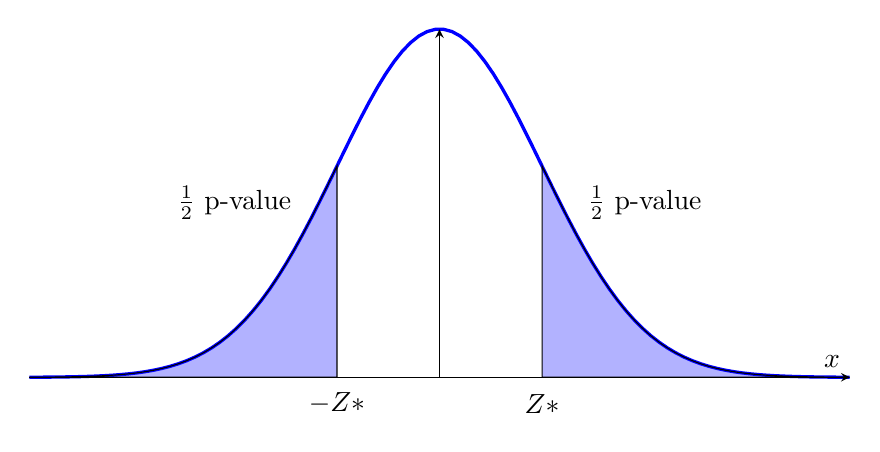
\begin{tikzpicture}
  \begin{axis}[
    no markers, domain=-4:4, samples=100,
    axis lines=middle,
    xlabel={$x$}, ylabel={},
    height=6cm, width=12cm,
    xtick=\empty,
    ytick=\empty,
    enlargelimits=false, clip=false,
    axis on top,
    grid = major,
  ]
    \addplot [very thick, blue] {1/sqrt(2*pi) * exp(-x^2/2)};
    \addplot [
      domain=-4:-1,
      samples=100,
      fill=blue,
      fill opacity=0.3,
    ]
    {1/sqrt(2*pi) * exp(-x^2/2)} \closedcycle;
    \addplot [
      domain=1:4,
      samples=100,
      fill=blue,
      fill opacity=0.3,
    ]
    {1/sqrt(2*pi) * exp(-x^2/2)} \closedcycle;

    % Labels for p-value regions
    \node at (axis cs:-2,0.2) {$\frac{1}{2}$ p-value};
    \node at (axis cs:2,0.2) {$\frac{1}{2}$ p-value};
    \node at (axis cs:1, -0.03) {$Z*$};
    \node at (axis cs:-1, -0.03) {$-Z*$};
  \end{axis}
\end{tikzpicture}
\end{center}
\caption{An illustration of hypothesis test on a proportion that $H_0: p = p_0$, $H_a: p \neq p_0$.}
\end{figure}

Note that when the alternative test is $H_a: p \neq p_0$, then we are going to consider the test hypothesis as a two-tailed test. Now, let's consider that the test statistics is a positive value, then: p-value $= P(X \ge Z^*) + P(X \le -Z^*) = 2 \cdot P(X \ge Z^*) = 2 \cdot  P(X \le -Z^*)$. Note that these different methods of calculation will give you same answer.\\

\textbf{Step 4: Comparing p-value with $\alpha$}

Same as before, if $p > \alpha$, then we do not reject the null hypothesis. Otherwise, we reject the null hypothesis and take the alternative hypothesis as our final conclusion.\\

\textbf{Step 5: Stating the final conclusion about the test}

P-value $< \alpha$ level, we reject $H_0$; we can conclude $H_a$ (we have evidence to support our claim). Often we phrase as a statistically significant result at that specified $\alpha$-level. P-value $> \alpha$-level, we fail to reject $H_0$; We cannot conclude $H_a$ (we have not enough evidence to support our claim); thus, $H_0$ is plausible, we do not accept $H_a$. Often we phrase as the result is not statistically significant at that specified $\alpha$-level.\\

\textbf{Conditions of One Sample Test Hypothesis on a Proportion}

\begin{itemize}
	\item 1. Random sample;
	\item 2. Independent sample;
	\item 3. If sample size $n < 30$, then population should be normal.
\end{itemize}

\section{One Sample Hypothesis Tests for a Variance}

Now, let's move to hypothesis tests for one variance, which follows the exact same idea from test hypothesis on proportion. We are going to introduce that by using steps as well.\\

\textbf{Step 1: Stating the Structure of Testing Hypothesis}

\begin{center}
\begin{figure}[H]
\centering
\begin{tabular}{ c c c }
Cases & Null Hypothesis & Alternative Hypothesis \\
     1	   & $H_0: \sigma^2 = \sigma_0^2$ & $H_a: \sigma^2 > \sigma_0^2$ \\
     2	   & $H_0: \sigma^2 = \sigma_0^2$ & $H_a: \sigma^2 < \sigma_0^2$ \\
     3    & $H_0: \sigma^2 = \sigma_0^2$ & $H_a: \sigma^2 \neq \sigma_0^2$ \\
\end{tabular}
\caption{All possible cases of one sample hypothesis test on a variance}
\end{figure}
\end{center}
\vspace{-2.00em}

\textbf{Step 2: Computing Test Statistics}

\begin{definition}[Test statistics of one sample hypothesis test on a variance]
The test statistics of one sample hypothesis test on a variance is given by: \[ \chi_*^2 = \frac{(n-1)s^2}{\sigma_0^2} \sim \chi_{n-1}^2.\]
Note that $n$ represents the sample size, $s^2$ is the sample variance of the chosen sample.
\end{definition}

\textbf{Step 3: Decision Rules}

\begin{itemize}
	\item 1. $H_0: \sigma^2 = \sigma_0^2$ and $H_a: \sigma^2 \neq \sigma_0^2$ (teo tailed alternative). We reject $H_0$ if $\chi_*^2 > \chi_{n-1;\alpha/2}^2$ or if $\chi_*^2 < \chi_{n-1;1-\alpha/2}^2$.
	\item 2. $H_0: \sigma^2 = \sigma_0^2$ and $H_a: \sigma^2 > \sigma_0^2$ (upper tailed alternative). We reject $H_0$ if $\chi_*^2 > \chi_{n-1;\alpha}^2$ or if $P[\chi_{n-1}^2 > \chi_*^2]$ is too small.
	\item 3. $H_0: \sigma^2 = \sigma_0^2$ and $H_a: \sigma^2 < \sigma_0^2$ (lower tailed alternative). We reject $H_0$ if $\chi_*^2 < \chi_{n-1;1-\alpha}^2$ or if $P[\chi_{n-1}^2 < \chi_*^2]$ is too small.
\end{itemize}

Note that this is not robust to departures from normality.


In case (i), calculating $P[Z > Z_*]$ as your p-value. Then, comparing with significant level: $\alpha$.

ii. When is structure of testing hypothesis is $H_0: p = p_0$, $H_a: p < p_0$:


In case (ii), calculating $P[Z < Z_*]$ as your p-value. Then, comparing with significant level: $\alpha$.

iii. When is structure of testing hypothesis is $H_0: p = p_0$, $H_a: p \neq p_0$:


In case (iii), calculating $2\cdot P[Z > |Z_*|]$ as your p-value. Then, comparing with significant level: $\alpha$.\\

\textbf{Step 4: Comparing P-value with $\alpha$-level}

If p-value is less than $\alpha$-level, then we reject the null hypothesis ($H_0$) and accept the alternative hypothesis ($H_a$). Otherwise, If p-value is greater than $\alpha$-level, then we do not reject the null hypothesis ($H_0$) and reject the alternative hypothesis ($H_a$).\\

\textbf{Step 5: Final Conclusion}
If we reject the null hypothesis, then we conclude that: there is sufficient evidence to reject the null hypothesis. If we do not reject the null hypothesis, then we conclude that: there is insufficient evidence to reject the null hypothesis.\\

\textbf{Conditions on One Sample Test Hypothesis on a Proportion}
\begin{itemize}
	\item 1. Random sample;
	\item 2. Independent sample: each observations are independent to others;
	\item 3. Sufficient sample.
\end{itemize}